\documentclass[12pt, a4paper, oneside]{ctexart}
\usepackage{amsmath, amsthm, amssymb, graphicx}
\usepackage{float}
\usepackage{diagbox}
\usepackage[bookmarks=true, colorlinks, citecolor=blue, linkcolor=black]{hyperref}

% tikz画图包
\usepackage{pgfplots}
\usetikzlibrary{patterns,arrows,positioning,calc,fadings,shapes,decorations.markings}
\usepackage{tikz}

% 导言区
\title{作业二第6题}
\author{崔俊杰}

\begin{document}
\maketitle
\raggedright(1)电路的输出方程:\(Y = Q_2\) \\
\quad \\
\raggedright(2)电路的驱动方程:
$
\begin{cases}

    D_0 = Q_2^{'}Q_1^{'}Q_0^{'} \\
    D_1 = Q_0 \\
    D_2 = Q_1 

\end{cases}
$\\ 
\quad \\
\raggedright(3)电路的状态方程:\\
由D触发器的特性方程\(Q = D\)有\\
\begin{align}
    Q_0 &= J_1Q_1^{'} + K_1^{'}Q_1 \nonumber \\
    &= Q_3^{'}Q_1^{'} + Q_3Q_1 \nonumber \\
    &= Q_3 \odot Q_1 \nonumber
\end{align}
\begin{align}
    Q_2 &= J_2Q_2^{'} + K_2^{'}Q_2 \nonumber \\
    &= Q_2^{'}Q_1 + Q_2Q_1^{'} \nonumber \\
    &= Q_2 \oplus Q_1 \nonumber
\end{align}
\begin{align}
    Q_3 &= J_3Q_3^{'} + K_3^{'}Q_3 \nonumber \\
    &= Q_3^{'}Q_2Q_1 + Q_3^{'}Q_3 \nonumber \\
    &= Q_3^{'}Q_2Q_1 \nonumber
\end{align}
\raggedright 故电路的状态方程为:
$
\begin{cases}
    Q_1 = Q_3 \odot Q_1 \\ 
    Q_2 = Q_2 \oplus Q_1 \\ 
    Q_3 = Q_3^{'}Q_2Q_1 \\
\end{cases}
$\\
\; \\
\; \\
\raggedright(4)电路的状态图如图所示: \\
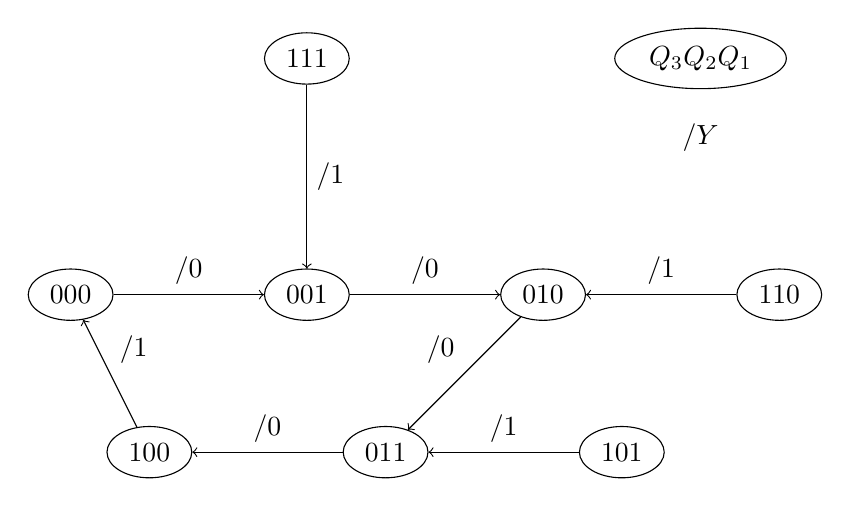
\begin{tikzpicture}
    \node (Y) at (10,0) {/$Y$};
    \node [draw,shape=ellipse](n1) at (2,-2) {000};
    \node [draw,shape=ellipse](n2) at (5,-2) {001};
    \node [draw,shape=ellipse](n3)at (8,-2) {010};
    \node [draw,shape=ellipse](n4)at (11,-2) {110};
    \node [draw,shape=ellipse](n5)at (3,-4) {100};
    \node [draw,shape=ellipse](n6)at (6,-4) {011};
    \node [draw,shape=ellipse](n7)at (9,-4) {101};
    \node [draw,shape=ellipse](n8)at (5,1) {111};
    \node [draw,shape=ellipse](n)at (10,1) {$Q_3Q_2Q_1$};

    \draw[->] (n1) -- node[above] {/0} (n2); 
    \draw[->] (n2) -- node[above] {/0} (n3); 
    \draw[->] (n4) -- node[above] {/1} (n3); 
    \draw[->] (n5) -- node[above right] {/1} (n1); 
    \draw[->] (n6) -- node[above] {/0} (n5); 
    \draw[->] (n7) -- node[above] {/1} (n6); 
    \draw[->] (n3) -- node[above left] {/0} (n6); 
    \draw[->] (n8) -- node[right] {/1} (n2);
\end{tikzpicture}
\\
\;\\
\textbf{由图可知,该电路可以自启动.} \\\;\\
\raggedright(5)分析电路的逻辑功能:\\
\textbf{由状态图可知,该电路实现的是一个时序模5计数器.}

\newpage

\begin{tikzpicture}
    \node [draw,shape=ellipse] (a) at (4,10) {IDLE};
    \node [draw,shape=ellipse] (b) at (8,10) {START};
    \node [draw,shape=ellipse] (c) at (12,10) {DATA};
    \node [draw,shape=ellipse] (d) at (16,10) {STOP};
    \node at (9.5,14) {back};

    \draw [->] (a) node at (4,7.5) {loop0}arc(90:-240:1);
    \draw [->] (b) node at (8,7.5) {loop1} arc(90:-240:1);
    \draw [->] (c) node at (12,7.5) {loop2} arc(90:-240:1);
    \draw [->] (a) -- node[above] {in1}(b);
    \draw [->] (b) -- node[above] {in2}(c);
    \draw [->] (c) -- node[above] {in3} (d);
    \draw [->] (d) to [in = 120,out = 90] (a);
\end{tikzpicture}
\\
\raggedright \textbf{说明}\\
1,状态说明: \\
IDLE : 空闲态 \\
START : 启动态 \\
DATA : 数据读取态 \\
STOP : 结束态 \\
2,条件说明:\\
in1 : din = 0 \\
in2 : \text{cnt\_baud = BAUD\_MAXN} \\
in3 : \text{end\_data = 1} \\
loop0 : \text{din = 1} \\
loop1 : \text{cnt\_baud != BAUD\_MAXN} \\
loop2 : \text{end\_data = 0} \\
back : \text{end\_cnt = BAUD\_MAXN}
\newpage


\begin{tikzpicture}

    %\draw[step=1,help lines] (-4,-10) grid (13, 10); 

    \draw (2,0) rectangle (5.5,5);
    \node (module_1) at(3.5,4.6) {SW\_send};

    \draw (2,-6) rectangle (5.5,-1);
    \node (module_2) at(3.5,-1.4) {led\_recv\_show};

    \draw (-1,-8) rectangle (8.5,7);
    \node (top_module) at(3.5,6.7) {top\_control};

    \node (S3) at(-3,4) {S3};
    \node (data) at(-3,3) {data};
    \node (clk) at(-3,2) {clk};
    \node (rst) at(-3,1) {rst};
    \node (uart_rx) at(-3,-5) {uart\_rx};
    \node (uart_tx) at(11,2.5) {uart\_tx};
    \node (en) at (11,-2.5) {en};
    \node (SEGS) at (11,-4.5) {SEGS};
    \node at (-1.7,3) {8/};
    \node at (10,-2.5) {8/};
    \node at (10,-4.5) {7/};

    \draw[-] (S3) to (2,4);
    \draw[-] (data) to (2,3);
    \draw[-] (clk) to (2,2);
    \draw[-] (rst) to (2,1);

    \draw[-] (uart_rx) to (2,-5);
    \draw[-] (-2,2) |- (2,-2);
    \draw[-] (-1.5,1) |- (2,-3.5);
    \fill (-2,2) circle (2pt);
    \fill (-1.5,1) circle (2pt);
    \draw (uart_tx) to (5.5,2.5);
    \draw (en) to (5.5,-2.5);
    \draw (SEGS) to (5.5,-4.5);
\end{tikzpicture}

\newpage

\begin{tikzpicture}
    %\draw[step=1,help lines] (-4,-10) grid (13, 10);
    
    \draw (2,0) rectangle (6,6);
    \draw (0,-2) rectangle (8,8);
    \node at (4,5.5) {calculator};
    \node at (4,7.5) {top\_calculator};

    \node (clk) at (-2,4.5) {clk};
    \node (rst) at (-2,3) {rst};
    \node (uart_rx) at (-2,1.5) {uart\_rx};
    \node (uart_tx) at (9.5,3) {uart\_tx};

    \draw[-] (clk) to (2,4.5);
    \draw[-] (rst) to (2,3);
    \draw[-] (uart_rx) to (2,1.5);
    \draw[-] (uart_tx) to (6,3);
    

\end{tikzpicture}
\end{document}